\chapter{Implementacija i korisničko sučelje}
		
		
		\section{Korištene tehnologije i alati}
		
			 U svrhu ovog projekta korištene su sljedeće tehnologije i alati: Django i Bootstrap web programski okviri, sustav za upravljanje bazom podataka PostGreSQL, program pgAdmin, jezici HTML, CSS i JavaScript te biblioteku jQuery. \\
			 
			 
			 {Za pisanje backenda korišten je Django, web programski okvir utemeljen na jeziku Python. Preuzeti se može na ovoj  \href{https://www.djangoproject.com/}{\textbf{poveznici}}.
			 	
			 Baza podataka ostvarena je kroz sustav \href{https://www.postgresql.org/}{\textbf{PostGreSQL}} te uz pomoć programa \href{https://www.pgadmin.org/}{\textbf{pgAdmin}}.
			 
			 Frontend dio ostvaren je kroz korištenje standardnih jezika \href{https://www.w3schools.com/html/}{\textbf{HTML}},\href{https://www.w3schools.com/css/}{\textbf{CSS}} te \href{https://www.w3schools.com/js/DEFAULT.asp}{\textbf{JavaScript}}. Linkovi vode na stranice gdje se o njima može više saznati. 
			 
			 Uz navedene jezike korišteni su i programski okvir \href{https://getbootstrap.com/}{\textbf{Bootstrap}} pomoću kojeg su dobivene neke napredne funkcionalnosti frontenda te biblioteke \href{https://jquery.com/}{\textbf{jQuery}}.
			
			
			\eject 
		
	
		\section{Ispitivanje programskog rješenja}
			
			
			Ispitivanje se provodilo ručno. Kao temelj za ispitivanje koristili su se obrasci uporabe. Osim preciznog praćenja obrazaca također smo i nasumično navigirali po stranici u slučaju da negdje postoje greške u kodu (bugovi). Iako smo provjerili cijeli sustav radi pojednostavljenja u dokumentaciji prikazujemo samo 6 ispitnih slučajeva. Ispitali smo: UC2, UC3, UC10, UC18, UC20, UC24
			\\
			\\ 
			\textbf{Ispitni slučaj 1: Detaljan pregled priča}
			\\
			\textbf{Ulaz}
			\\
			\indent 1. Pritisak kursorom na određenu priču
			\\
			\textbf{Očekivani rezultat}
			\\
			\indent 1. Preusmjeravanje na stranicu odabrane priče
			\\
			\textbf{Rezultat}
			\\
			\indent Očekivani rezultat je zadovoljen te smo preusmjereni na stranicu za detaljan pregled priče koje smo odabrali. Slučaj je testiran i kao prijavljen korisnik i kao gost. Aplikacija je prošla test.
			\\ \\
			\begin{figure}[H]
				\centering
				\includegraphics[scale=0.34]{"slike/test1"}
				\caption{Rezultat ispitnog slučaja 1}
				\label{fig:rezultat-ispitnog-slucaja-1}
			\end{figure}
			
			\noindent \textbf{Ispitni slučaj 2: Komentiranje priče}
			\\
			\textbf{Ulaz}
			\\
			\indent 1. Navigacija do detaljnog pregleda priče \\
			\indent 2. Upisivanje samog komentara u predviđeno mjesto \\
			\indent 3. Pritisak gumba "Objavi"
			\\
			\textbf{Očekivani rezultat}
			\\
			\indent 1. Spremanje komentara u bazu za kasniji prikaz na stranici priče \\
			\indent 2. Osvježavanje stranice
			\\
			\textbf{Rezultat}
			\\
			\indent Očekivani rezultat je zadovoljen te se stranica osvježila te vidimo komentar koji smo ostavili. Komentar smo uspješno ostavili i kao gost i kao prijavljeni korisnik. Aplikacija je prošla test.
			\\ \\
			\begin{figure}[H]
				\centering
				\includegraphics[scale=0.34]{"slike/test2"}
				\caption{Rezultat ispitnog slučaja 2}
				\label{fig:rezultat-ispitnog-slucaja-2}
			\end{figure}
			
			\noindent \textbf{Ispitni slučaj 3: Predlaganje priče administratoru}
			\\
			\textbf{Ulaz}
			\\
			\indent 1. Navigacija stranice za prijedlog priče \\
			\indent 2. Odabir medije, naslova zahtjeva i naslova priče \\
			\indent 3. Pritisak gumba "Predloži priču"
			\\
			\textbf{Očekivani rezultat}
			\\
			\indent 1. Spremanje prijedloga priče u bazu \\
			\indent 2. Preusmjeravanje na stranicu sandučića
			\\
			\textbf{Rezultat}
			\\
			\indent Očekivani rezultat je zadovoljen. Preusmjereni smo na stranicu sandučića na kojoj vidimo još neobrađen zahtjev naše priče. Aplikacija je prošla test.
			\\ \\
			\begin{figure}[H]
				\centering
				\includegraphics[scale=0.34]{"slike/test3"}
				\caption{Rezultat ispitnog slučaja 3}
				\label{fig:rezultat-ispitnog-slucaja-3}
			\end{figure}
			
			\noindent \textbf{Ispitni slučaj 4: Pregled košarice}
			\\
			\textbf{Ulaz}
			\\
			\indent 1. Pritisak na gumb "Košarica" \\
			\textbf{Očekivani rezultat}
			\\
			\indent 1. Prikaz sadržaja u košarici, ukupne cijene te gumba za dovršavanje narudžbe. \\
			\textbf{Rezultat}
			\\
			\indent Očekivani rezultat je zadovoljen. Pritiskom na gumb košarica otvora se prikaz već navedenog sadržaja. Aplikacija je prošla test.
			\\ \\
			\begin{figure}[H]
				\centering
				\includegraphics[scale=0.34]{"slike/test4"}
				\caption{Rezultat ispitnog slučaja 4}
				\label{fig:rezultat-ispitnog-slucaja-4}
			\end{figure}
			
			\noindent \textbf{Ispitni slučaj 5: Promjena profilne slike}
			\\
			\textbf{Ulaz}
			\\
			\indent 1. Navigacija do stranice profila \\
			\indent 2. Odabir datoteke na računalu \\
			\indent 3. Pritisak gumba "Promijeni profilnu sliku" \\
			\textbf{Očekivani rezultat}
			\\
			\indent 1. Osvježavanje trenutne stranice na kojoj vidimo da je profilna slika promijenjena \\
			\textbf{Rezultat}
			\\
			\indent Očekivani rezultat nije zadovoljen. Namjerno nije odabrana nijedna slika, a gumb je svejedno pritisnut. Stranica se osvježila te profilna slika nije ažurirana.
			\\ \\
			\begin{figure}[H]
				\centering
				\includegraphics[scale=0.34]{"slike/test5"}
				\caption{Rezultat ispitnog slučaja 5}
				\label{fig:rezultat-ispitnog-slucaja-5}
			\end{figure}
			
			\noindent \textbf{Ispitni slučaj 6: Pregled registriranih korisnika}
			\\
			\textbf{Ulaz}
			\\
			\indent 1. Pritisak na ime korisnika bilo gdje na stranici \\
			\textbf{Očekivani rezultat}
			\\
			\indent 1. Prikaz profila odabranog korisnika. \\
			\textbf{Rezultat}
			\\
			\indent Očekivani rezultat je zadovoljen. Pritiskom na korisničko ime u komentarima preusmjereni smo na pregled profila odabranog korisnika. Aplikacija je prošla test.
			\\ \\
			\begin{figure}[H]
				\centering
				\includegraphics[scale=0.34]{"slike/test6"}
				\caption{Rezultat ispitnog slučaja 6}
				\label{fig:rezultat-ispitnog-slucaja-6}
			\end{figure}
			
			
		\subsection{Ispitivanje sustava}
			
			 
			 Korištenjem extenzije za Chrome preglednik Selenium isprobali smo sljedeće obrasce uporabe UC7, UC11, UC19 i UC4.
			 \\
			 \noindent \textbf{Ispitni slučaj 1: Pregled web shopa kao administrator}
			 \\
			 \textbf{Ulaz}
			 \\
			 \indent 1. Odabir gumba za prikaz webshopa iz padajućeg izbornika na zaglavlju stranice \\
			 \textbf{Očekivani rezultat}
			 \\
			 \indent 1. Prikaz webshopa. \\
			 \textbf{Rezultat}
			 \\
			 \indent Očekivani rezultat je zadovoljen. Pritiskom na spomenuti gumb preusmjereni smo na stranicu webshopa. Na slici je prikazano izvršavanje testa
			 \\ \\
			 \begin{figure}[H]
			 	\centering
			 	\includegraphics[scale=0.7]{"slike/test7"}
			 	\caption{Rezultat ispitnog slučaja 1}
			 	\label{fig:rezultat-ispitnog-slucaja-7}
			 \end{figure}
			 
			 \noindent \textbf{Ispitni slučaj 2: Ocjenjivanje priče}
			 \\
			 \textbf{Ulaz}
			 \\
			 \indent 1. Navigacija do stranice neke priče \\
			 \indent 2. Odabir opcije "sviđa mi se"/"ne sviđa mi se" \\
			 \textbf{Očekivani rezultat}
			 \\
			 \indent 1. Osvježenje stranice i ažuriranje broja ocjena priče\\
			 \textbf{Rezultat}
			 \\
			 \indent Očekivani rezultat je zadovoljen. Navigirali smo se do stranice priče i odabrali opciju "sviđa mi se" kao prijavljeni korisnik. Na slici je prikazano izvršavanje testa
			 \\ \\
			 \begin{figure}[H]
			 	\centering
			 	\includegraphics[scale=0.7]{"slike/test8"}
			 	\caption{Rezultat ispitnog slučaja 2}
			 	\label{fig:rezultat-ispitnog-slucaja-8}
			 \end{figure}
			 
			 \noindent \textbf{Ispitni slučaj 3: Upravljanje postavkama o privatnosti}
			 \\
			 \textbf{Ulaz}
			 \\
			 \indent 1. Navigacija do stranice vlastitog profila \\
			 \indent 2. Mijenjanje postavka privatnosti" \\
			 \indent 3. Pritisak gumba "Spremi postavke privatnosti" \\
			 \textbf{Očekivani rezultat}
			 \\
			 \indent 1. Osvježenje stranice i ažuriranje postavka privatnosti\\
			 \textbf{Rezultat}
			 \\
			 \indent Očekivani rezultat je zadovoljen. Navigirali smo se do stranice vlastitog profila i postavili adresu elektroničke pošte da bude privatna. Na slici je prikazano izvršavanje testa
			 \\ \\
			 \begin{figure}[H]
			 	\centering
			 	\includegraphics[scale=0.7]{"slike/test9"}
			 	\caption{Rezultat ispitnog slučaja 3}
			 	\label{fig:rezultat-ispitnog-slucaja-9}
			 \end{figure}
			 
			 \noindent \textbf{Ispitni slučaj 4: Registracija korisnika}
			 \\
			 \textbf{Ulaz}
			 \\
			 \indent 1. Navigacija do stranice za registraciju \\
			 \indent 2. Upisivanja podataka" \\
			 \indent 3. Pritisak gumba "Kreiraj račun" \\
			 \textbf{Očekivani rezultat}
			 \\
			 \indent 1. Registracija korisnika\\
			 \indent 2. Preusmjeravanje na početnu stranicu
			 \textbf{Rezultat}
			 \\
			 \indent Očekivani rezultat nije zadovoljen. Izostavili smo korisničko ime pri ispunjavanju podataka. Iskočila je poruka upozorenja da se to polje popuni. Na slici je prikazan krajnji dio izvršavanja testa.
			 \\ \\
			 \begin{figure}[H]
			 	\centering
			 	\includegraphics[scale=0.7]{"slike/test10"}
			 	\caption{Rezultat ispitnog slučaja 4}
			 	\label{fig:rezultat-ispitnog-slucaja-10}
			 \end{figure}
		
		
		\section{Dijagram razmještaja}
			
			Sustav je baziran na arhitekturi "klijent-poslužitelj". Koristimo HTTP za komunikaciju između korisnikovog uređaja i poslužitelja. Za posluživanje koristimo Heroku koji nudi platformu kao uslugu u oblaku. Heroku se sam brine o portovima, operativnim sustavima i okolinama poslužitelja pa nisu prikazani u dijagramu.
			
			\begin{figure}[!h]
				\centering
				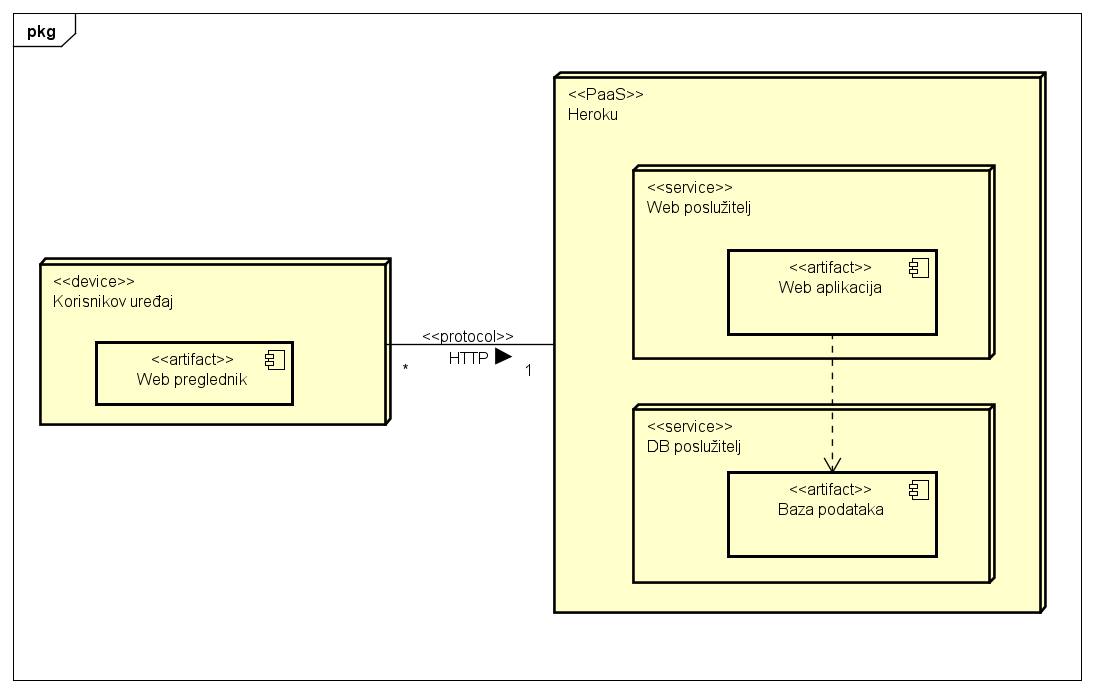
\includegraphics[width=1\linewidth]{slike/Dijagram_razmjestaja}
				\caption{Dijagram razmještaja}
				\label{fig:dijagramrazmjestaja}
			\end{figure}
			\eject
			
			\eject 
		
		\section{Upute za puštanje u pogon}
			\textbf{Instalacija Heroku poslužitelja}\\
			\\
			Potrebno je imati lokalno instalirani python verzije 3.8
			zajedno s najnovijom verzijom Django-a, najnoviju verziju Postgres-a, Git te besplatni Heroku račun.
			Potrebno je preuzeti Heroku Command Line Interface (CLI) koji je dostupan na https://cli-assets.heroku.com/heroku-x64.exe.
			Nakon toga potrebno je u Windows Command Prompt-u (cmd.exe) pokrenuti
			naredbu \verb|heroku login| koja će u zasebnom prozoru preglednika prikazati stranicu za login. \\
			\\
			\textbf{Konfiguracija aplikacije za Heroku}\\
			\\
			Kako bi se Heroku web aplikacija dobro konfigurirala potrebno je u
			Django server dodati 3 datoteke: \\
			1) requirements.txt s \\
			"Django==3.1.3 \\
			gunicorn==20.0.4 \\
			psycopg2-binary==2.8.6 \\
			pytz==2020.4 \\
			sqlparse==0.4.1 \\
			asgiref==3.3.0 \\
			dj-database-url==0.5.0 \\
			whitenoise==5.2.0 \\
			boto3==1.16.51 \\
			botocore==1.19.51 \\
			django-storages==1.11.1 \\
			jmespath==0.10.0 \\
			python-dateutil==2.8.1 \\
			s3transfer==0.3.3 \\
			six==1.15.0 \\
			urllib3==1.26.2" \\
			\\
			2) Procfile (bitno: Datoteka nema ekstenziju) s \\
			"web: gunicorn WeTried.wsgi --log-file -"
			\\
			3) runtime.txt s \\
			"python-3.8.6" \\
			\\
			\textbf{Stvaranje Heroku web aplikacije}\\
			\\
			Potrebno je imati lokalni git repozitorij koji se može stvoriti naredbom
			\verb|git init|.
			Pokretanjem naredbe 
			\verb|heroku create <name>| (naš name glasi "maketashop")
			stvara se heroku aplikacija i automatski se povezuje s lokalnim git repozitorijem.
			Nakon stvaranja aplikacije potrebno je dostaviti sam server pomoću naredbe \verb|git push heroku master|. Ako proces završi bez grešaka aplikacija je uspješno puštena u pogon, ostalo je samo povezati bazu s Djangom.
			\\
			\\
			\textbf{Konfiguriranje baze podataka}\\
			\\
			Heroku sam po sebi pri stvaranju python web aplikacije stvori addon
			postgresql tako da je potrebno samo u settings.py dodati \\
			\verb|"DATABASE_URL = <url>"| (url koji je generirao heroku) \\
			"DATABASES = {
				'default': dj\_database\_url.config(default=DATABASE\_URL)
			}"
			i \\
			"ALLOWED\_HOSTS = ['maketashop.herokuapp.com']". \\
			Nemojte zaboraviti maknuti konfiguraciju za korištenje lokalne baze podataka.\\
			\\
			\textbf{Upravljanje bazom podataka}\\
			\\
			Prije korištenja baze podataka potrebno je napraviti migracije te ih pokrenuti kako bi u bazi podataka bile sve tablice koje su potrebne za funkcioniranje baze podataka. To se radi tako što pokrenemo \verb|heroku run python manage.py makemigrations| koja napravi migracije, a zatim \verb|heroku run python manage.py migrate| koja te migracije primijeni.
			
			Budući da aplikacija velikim dijelom nema sadržaja dok korisnici ne počnu postavljati sadržaj, nije potrebno nikako populirati bazu podataka
			
			Da bismo vidjeli koji dodatak koristimo kako bismo se spojili na bazu podataka, pokrećemo naredbu \verb|heroku addons| koja nam daje sljedeći ispis:
			\begin{figure}[H]
				\centering
				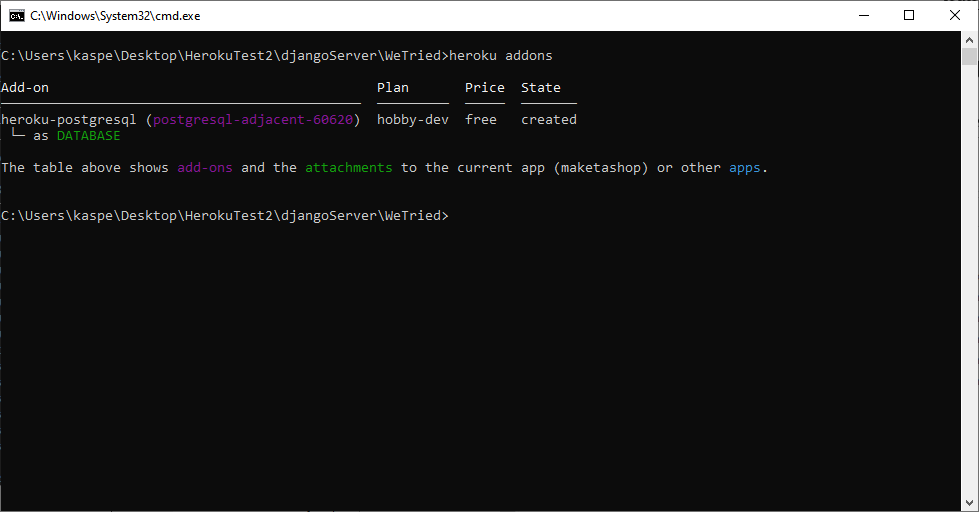
\includegraphics[width=1\linewidth]{slike/herokuPostgresql}
				\caption{Ispis naredbe heroku addons}
				\label{fig:herokuaddons}
			\end{figure}
			
			Ako želimo izravno upravljati bazom koristeći SQL upite kao vlasnik aplikacije, u naredbenom retku pokrećemo naredbu \verb|heroku pg:psql| koja nam otvara sučelje u kojemu možemo upisivati upite.
			
			\begin{figure}[H]
				\centering
				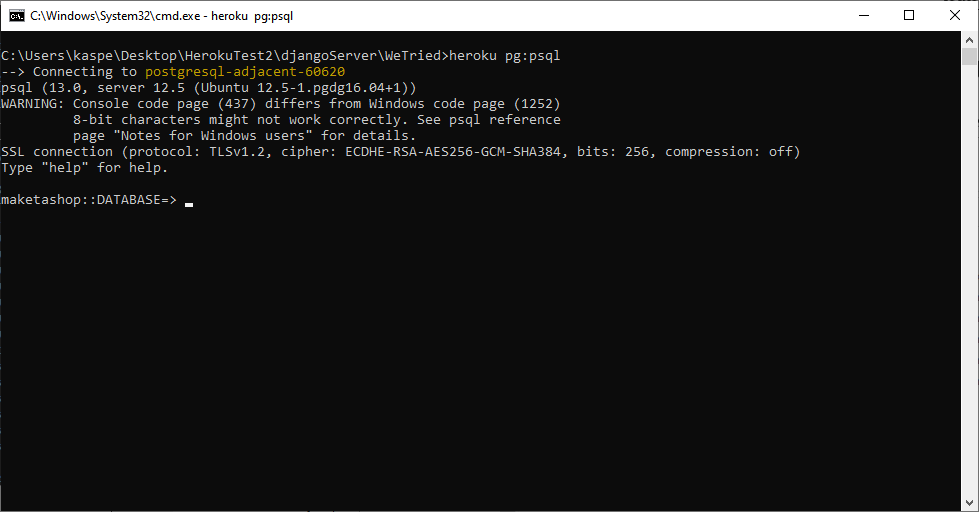
\includegraphics[width=1\linewidth]{slike/herokuPostgresql2}
				\caption{Ispis naredbe heroku pg:psql}
				\label{fig:pgpsql}
			\end{figure}
			Kada smo gotovi s postavljanjem upita, iz sučelja izlazimo naredbom \verb|\q|\\
			\\
			\textbf{Postavljanje posluživanja statičkih resursa}
			\\
			\\
			Budući da Django ne podržava posluživanje statičkih resursa u produkciji, potrebno je instalirati i konfigurirati paket whitenoise. Paket će biti instaliran budući da smo ga uključili u requirements.txt. Potrebno je još dodati sljedeće postavke u settings.py datoteku:\\
			\verb|BASE_DIR = os.path.dirname(os.path.dirname(os.path.abspath(__file__)))|\\
			\verb|STATIC_ROOT = os.path.join(BASE_DIR, 'staticfiles')|\\
			\verb|STATIC_URL = '/static/'|
			\begin{verbatim}
				STATICFILES_DIRS = (
					os.path.join(BASE_DIR, 'static'),
				)
			\end{verbatim}
			Osim toga, potrebno je dodati whitenoise middleware u MIDDLEWARE listu u datoteci settings.py. To seradi tako što samo dodamo string\\ \verb|'whitenoise.middleware.WhiteNoiseMiddleware',|\\ odmah nakon sigurnosnog middlewarea.
			\\
			\\
			\textbf{Postavljanje posluživanja korisničkih datoteka}
			\\
			\\
			Veliki dio funkcionalnosti aplikacije oslanja se na mogućnost korisnika da postavljaju svoje datoteke na server. Primjer toga je recimo sastavljanje priče ili kreiranje makete u web trgovini za koju je potrebno definirati sliku. Kako je heroku-ov datotečni sustav kratkotrajan (eng. \textit{ephemeral filesystem}), datoteke je potrebno spremiti na udaljeni poslužitelj i dohvaćati ga od tamo.\\
			Kako bismo ostvarili tu funkcionalnost odlučili smo koristiti Amazonov web servis S3. Da bi mogli spojiti se na AWS S3, potrebno je instalirati paket django-storages, zbog cega je on vec dodan u requirements.txt file, što znači da će biti instaliran prilikom puštanja aplikacije u pogon.\\
			Također, potrebno je registrirati se na amazonov servis. Na glavnoj stranici Amazon Web Services (\url{https://aws.amazon.com}), nalazi se gumb koji možemo kliknuti i unijeti podatke potrebne za registraciju. Nakon registracije. Kada pronađemo stranicu usluge S3, kreiramo 
			\eject 